% =====================================================================
\newpage
\part{Segundo Parcial 2025}
% =====================================================================
\section{Parcial 2025 --- Tema 1}

% ---------------------------------------------------------------------
\subsection{Ejercicio 1 --- Distribución conjunta con regla de parada}
\begin{enun}
Una red tiene 10 nodos: 5 activos (A), 3 en reposo (R) y 2 desconectados (D). Se observan de a uno, sin reposición, y se para cuando (1) se observaron 3 nodos o (2) se observa el primer nodo no activo. $X$ = número de nodos activos observados; $Y$ = número de nodos en reposo observados.
a) Matriz $p(x,y)$. \ b) $\Cov(X,Y)$; ¿independientes? \ c) Si hay al menos un activo observado, probabilidad de que se haya registrado un nodo desconectado (y su expresión en términos de $X$ e $Y$).
\end{enun}
\begin{metodo}
Las observaciones son \textbf{sin reposición}, así que cada paso es una probabilidad condicional y se usa la \textbf{regla del producto}: $P(A_1\cap A_2\cap A_3)=P(A_1)\,P(A_2|A_1)\,P(A_3|A_1A_2)$.
\textbf{No} es una hipergeométrica con $n=3$ fijo: la cantidad de nodos observados depende de la regla de parada. Por eso hay que listar todas las \textbf{secuencias posibles} (diagrama de árbol) y asignar a cada una su par $(x,y)$.
\end{metodo}

\inciso{a) Matriz de probabilidad conjunta}
\paso{Paso 1 --- Secuencias posibles.} La observación termina en cuanto aparece un nodo no activo (R o D), o al llegar al tercero si todos fueron activos:
\begin{center}
\renewcommand{\arraystretch}{1.25}
\begin{tabular}{@{}lllcc@{}}
\toprule
Secuencia & Cálculo & Probabilidad & $x$ & $y$\\\midrule
R & $\frac{3}{10}$ & $0{,}3000$ & 0 & 1\\
D & $\frac{2}{10}$ & $0{,}2000$ & 0 & 0\\
A R & $\frac{5}{10}\cdot\frac{3}{9}=\frac{15}{90}=\frac16$ & $0{,}1667$ & 1 & 1\\
A D & $\frac{5}{10}\cdot\frac{2}{9}=\frac{10}{90}=\frac19$ & $0{,}1111$ & 1 & 0\\
A A R & $\frac{5}{10}\cdot\frac{4}{9}\cdot\frac{3}{8}=\frac{60}{720}=\frac1{12}$ & $0{,}0833$ & 2 & 1\\
A A D & $\frac{5}{10}\cdot\frac{4}{9}\cdot\frac{2}{8}=\frac{40}{720}=\frac1{18}$ & $0{,}0556$ & 2 & 0\\
A A A & $\frac{5}{10}\cdot\frac{4}{9}\cdot\frac{3}{8}=\frac{60}{720}=\frac1{12}$ & $0{,}0833$ & 3 & 0\\\bottomrule
\end{tabular}
\end{center}
\paso{Paso 2 --- Control.} $\frac3{10}+\frac2{10}+\frac16+\frac19+\frac1{12}+\frac1{18}+\frac1{12}=\frac{54+36+30+20+15+10+15}{180}=1$. \checkmark

\paso{Paso 3 --- Tabla de doble entrada} (cada celda suma las secuencias con ese par):
\begin{center}
\renewcommand{\arraystretch}{1.3}
\begin{tabular}{@{}c|cc|c@{}}
\toprule
$p(x,y)$ & $y=0$ & $y=1$ & $p_X(x)$\\\midrule
$x=0$ & $1/5=0{,}2000$ & $3/10=0{,}3000$ & $\mathbf{0{,}5000}$\\
$x=1$ & $1/9=0{,}1111$ & $1/6=0{,}1667$ & $\mathbf{0{,}2778}$\\
$x=2$ & $1/18=0{,}0556$ & $1/12=0{,}0833$ & $\mathbf{0{,}1389}$\\
$x=3$ & $1/12=0{,}0833$ & $0$ & $\mathbf{0{,}0833}$\\\midrule
$p_Y(y)$ & $\mathbf{0{,}4500}$ & $\mathbf{0{,}5500}$ & 1\\\bottomrule
\end{tabular}
\end{center}
La celda $(3,1)$ vale 0: si se observaron 3 activos ya se ocuparon los 3 lugares y no puede haber un nodo en reposo.

\inciso{b) Covarianza e independencia}
\paso{Paso 1 --- Esperanzas marginales.}
$\E(X)=0(0{,}5)+1\big(\tfrac{5}{18}\big)+2\big(\tfrac{5}{36}\big)+3\big(\tfrac1{12}\big)=\tfrac{29}{36}=0{,}8056$; \quad
$\E(Y)=0{,}5500$.

\paso{Paso 2 --- $\E(XY)$.} Solo aportan las celdas con $x\,y\neq0$: \ $\E(XY)=1\cdot1\cdot\tfrac16+2\cdot1\cdot\tfrac1{12}=\tfrac13=0{,}3333$.

\paso{Paso 3 --- Covarianza.}
\[
\Cov(X,Y)=\E(XY)-\E(X)\E(Y)=\frac13-\frac{29}{36}\cdot\frac{11}{20}=\frac{240-319}{720}=\res{-\frac{79}{720}=-0{,}1097}
\]
\paso{Paso 4 --- Independencia.} Si fueran independientes, la covarianza sería 0. Como $\Cov\neq0$, \textbf{no son independientes}. También alcanza con una celda: $p(3,1)=0\neq p_X(3)\,p_Y(1)=0{,}0833\cdot0{,}55=0{,}0458$.

\inciso{c) Probabilidad condicional}
\paso{Paso 1 --- Traducir el evento.} Como la observación se corta en el primer nodo no activo, se registra \emph{a lo sumo un} nodo no activo. Se registró un desconectado si y solo si se paró por un nodo no activo (o sea, $X\le2$) que no estaba en reposo ($Y=0$):
\[
\{\text{se registró un D}\}=\{Y=0,\ X\le2\}.
\]
\paso{Paso 2 --- Probabilidad pedida.}
\begin{align*}
P\big(Y=0,\ X\le2\ \big|\ X\ge1\big)&=\frac{P(Y=0,\ 1\le X\le2)}{P(X\ge1)}=\frac{p(1,0)+p(2,0)}{1-p_X(0)}\\
&=\frac{\frac19+\frac1{18}}{\frac12}=\frac{1/6}{1/2}=\res{\frac13=0{,}3333}
\end{align*}
\begin{ojo}
$X=3$ con $Y=0$ \textbf{no} cuenta: en ese caso se observaron 3 activos y ningún desconectado.
\end{ojo}

% ---------------------------------------------------------------------
\subsection{Ejercicio 2 --- Verdadero o falso}
\begin{enun}
a) $\Cov(h-X,\,X)<0$ para todo $h\in\mathbb{R}$ constante y cualquiera sea la distribución de $X$.
b) Los límites del IC para la varianza de una población normal son equidistantes de la varianza muestral.
\end{enun}
\inciso{a) FALSA}
\paso{Cálculo.} Por definición, y con $\mu=\E(X)$:
\begin{align*}
\Cov(h-X,X)&=\E[(h-X)X]-\E(h-X)\E(X)=h\mu-\E(X^2)-(h-\mu)\mu\\
&=-\big[\E(X^2)-\mu^2\big]=-\V(X).
\end{align*}
(Con propiedades: $\Cov(h-X,X)=\Cov(h,X)-\Cov(X,X)=0-\V(X)$.)

\paso{Conclusión.} $\Cov(h-X,X)=-\V(X)\le0$, y vale \textbf{cero} cuando $\V(X)=0$.
\begin{resp}
\textbf{Falsa.} Contraejemplo: $X$ degenerada, $P(X=c)=1$. Entonces $\V(X)=0$ y $\Cov(h-X,X)=0$, que no es $<0$.
Además, si $X$ no tiene varianza finita (por ejemplo, la distribución de Cauchy), la covarianza ni siquiera existe. La desigualdad estricta vale solo para $X$ no degenerada con varianza finita.
\end{resp}

\inciso{b) FALSA}
\paso{Planteo.} Para población normal, $\frac{(n-1)S^2}{\sigma^2}\sim\chis_{n-1}$, y el IC es
\[
L_1=\frac{(n-1)s^2}{\chis_{\alpha/2,\,n-1}},\qquad L_2=\frac{(n-1)s^2}{\chis_{1-\alpha/2,\,n-1}}.
\]
Para que fueran equidistantes de $s^2$ haría falta $s^2-L_1=L_2-s^2$, lo que exigiría una distribución simétrica. La $\chis$ es \textbf{asimétrica} (a derecha), así que eso no ocurre.

\paso{Contraejemplo numérico.} $n=10$, $s^2=1$, 95\,\%: \ $\chis_{0,025;9}=19{,}0228$ y $\chis_{0,975;9}=2{,}7004$.
\[
L_1=\frac{9}{19{,}0228}=0{,}4731,\qquad L_2=\frac{9}{2{,}7004}=3{,}3329.
\]
Distancias a $s^2=1$: $1-0{,}4731=0{,}5269$ y $3{,}3329-1=2{,}3329$. \textbf{No son iguales.}
\begin{resp}
\textbf{Falsa.} El IC para $\sigma^2$ no es simétrico alrededor de $s^2$, porque la distribución $\chis$ es asimétrica. El extremo superior queda mucho más lejos.
\end{resp}

% ---------------------------------------------------------------------
\subsection{Ejercicio 3 --- Prueba para una proporción}
\begin{enun}
Una empresa afirma que \emph{al menos} el 85\,\% de sus pedidos llega a tiempo, y solo tomará medidas correctivas si encuentra pruebas significativas de que no es así. En una muestra de 200 pedidos, 40 no llegaron a tiempo.
a) Hipótesis, estadístico y región de rechazo con $\alpha=0{,}05$. \ b) Conclusión, error posible y valor $P$. \ c) Elegir la curva de $\beta$. \ d) IC 95\,\% para la proporción a tiempo y comparación con b). \ e) $n$ para un error máximo de 3 puntos porcentuales con 95\,\%.
\end{enun}
\begin{metodo}
Prueba para una proporción con muestra grande. $X_i=1$ si el pedido $i$ llega a tiempo ($X_i\sim$ Bernoulli$(p)$), y $\hat P=\frac1n\sum X_i$.
Por el \textbf{TCL} (De Moivre--Laplace), $\hat P\approx\Nor\big(p;\,p(1-p)/n\big)$, válido porque $np_0=170\ge5$ y $n(1-p_0)=30\ge5$.
\end{metodo}

\inciso{a) Planteo de la prueba}
\paso{Datos.} $n=200$; a tiempo: $200-40=160$, así que $\hat p=160/200=0{,}80$.

\paso{Hipótesis.} La afirmación ``al menos 85\,\%'' se mantiene salvo evidencia en contra; las medidas correctivas se toman solo si se prueba lo contrario. Entonces la afirmación va en $H_0$ y la sospecha en $H_1$:
\[
H_0:\ p=0{,}85\ \ (p\ge0{,}85)\qquad\text{vs.}\qquad H_1:\ p<0{,}85.
\]
\paso{Estadístico de prueba} (bajo $H_0$ el desvío se calcula con $p_0$):
\[
Z=\frac{\hat P-p_0}{\sqrt{p_0(1-p_0)/n}}\ \overset{H_0}{\approx}\ \Nor(0;1),\qquad \sqrt{\frac{0{,}85\cdot0{,}15}{200}}=0{,}0252.
\]
\paso{Región de rechazo} (prueba unilateral izquierda): $Z<-z_{0,05}=-1{,}6449$. En unidades de $\hat p$: \ $\hat p<0{,}85-1{,}6449\,(0{,}0252)=\res{0{,}8085}$.

\inciso{b) Conclusión, error posible y valor $P$}
\[
z_0=\frac{0{,}80-0{,}85}{0{,}0252}=\res{-1{,}9803}<-1{,}6449\ \Rightarrow\ \textbf{se rechaza }H_0.
\]
\begin{resp}
Con $\alpha=0{,}05$ hay evidencia significativa de que menos del 85\,\% de los pedidos llega a tiempo: la empresa debería tomar medidas correctivas.
\textbf{Error posible:} como se rechazó $H_0$, el riesgo es un \textbf{error de tipo I}: concluir que no se cumple el 85\,\% (y tomar medidas correctivas innecesarias) cuando en realidad sí se cumple. Su probabilidad es como máximo $\alpha=0{,}05$.
\textbf{Valor $P$:} $P=P(Z\le-1{,}9803)=\Phi(-1{,}9803)=\res{0{,}0238}<0{,}05$, así que se rechaza: coincide con la decisión anterior. Con $\alpha=0{,}01$ no se rechazaría.
\end{resp}

\inciso{c) Curva de probabilidad de error tipo II}
\paso{Fórmula.} No se rechaza si $\hat p\ge0{,}8085$. Si la proporción verdadera es $p$, el desvío de $\hat P$ es $\sqrt{p(1-p)/n}$:
\[
\beta(p)=P(\hat P\ge0{,}8085\,|\,p)=1-\Phi\Big(\frac{0{,}8085-p}{\sqrt{p(1-p)/200}}\Big).
\]
\paso{Valores.}
\begin{center}
\begin{tabular}{@{}lccccc@{}}
\toprule
$p$ & 0,79 & 0,81 & 0,83 & 0,85 & 0,87\\\midrule
$\beta(p)$ & 0,2607 & 0,5220 & 0,7912 & 0,9500 & 0,9952\\\bottomrule
\end{tabular}
\end{center}
\begin{figure}[h]
\centering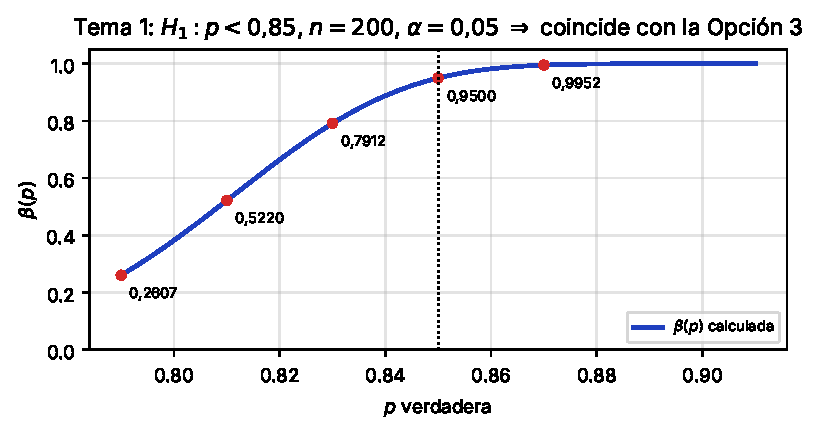
\includegraphics[width=0.78\textwidth]{fig/t1beta.pdf}
\end{figure}
\begin{resp}
\textbf{Opción 3.} La curva es \textbf{creciente} (la prueba es unilateral izquierda), vale $1-\alpha=0{,}95$ en $p_0=0{,}85$, tiende a 1 para $p>0{,}85$ y pasa por $(0{,}79;\,0{,}26)$, como la calculada.
Se descartan: 2 y 5 (forma de campana: corresponden a una prueba bilateral); 1 y 4 (decrecientes: corresponderían a $H_1:p>0{,}85$); 6 (creciente, pero en $p=0{,}79$ vale $\approx0{,}36$ y no $0{,}26$, y ya está casi en 1 en $p=0{,}85$ cuando debería valer $0{,}95$).
\end{resp}

\inciso{d) IC del 95\,\% para la proporción de pedidos a tiempo}
\paso{Planteo.} $n$ es grande, así que por el TCL se usa $\hat p\pm z_{0,025}\sqrt{\hat p(1-\hat p)/n}$. En el IC se usa $\hat p$ (no $p_0$), porque no se supone ningún valor de $p$.
\[
0{,}80\pm1{,}96\sqrt{\frac{0{,}8\cdot0{,}2}{200}}=0{,}80\pm1{,}96\,(0{,}0283)=0{,}80\pm0{,}0554\ \Rightarrow\ \res{0{,}7446\le p\le0{,}8554}
\]
\paso{Comparación con b).} El IC \emph{bilateral} contiene a 0,85, pero la prueba rechazó $H_0$. \textbf{No hay contradicción}, por dos motivos:
\begin{enumerate}
\item La prueba es \emph{unilateral} con $\alpha=0{,}05$. Lo que le corresponde es la \textbf{cota superior} del 95\,\%: $p\le0{,}80+1{,}6449\,(0{,}0283)=0{,}8465<0{,}85$, que sí excluye a 0,85, coherente con el rechazo.
\item En la prueba el error estándar se calcula con $p_0$ (0,0252) y en el IC con $\hat p$ (0,0283). Para proporciones, la dualidad IC--prueba es solo aproximada.
\end{enumerate}

\inciso{e) Tamaño de muestra para un error máximo $E=0{,}03$ con 95\,\%}
\paso{Fórmula.} De $E=z_{\alpha/2}\sqrt{p(1-p)/n}$ se despeja $n=\dfrac{z_{\alpha/2}^2\,p(1-p)}{E^2}$.

\paso{Para garantizarlo para cualquier $p$.} Como $p(1-p)\le\frac14$ (el máximo está en $p=\frac12$):
\[
n=\frac{1{,}96^2\cdot0{,}25}{0{,}03^2}=1067{,}1\ \Rightarrow\ \res{n=1068}
\]
\paso{Usando la estimación previa $\hat p=0{,}80$.} $n=\frac{1{,}96^2\cdot0{,}8\cdot0{,}2}{0{,}03^2}=682{,}95\Rightarrow683$.
\begin{resp}
Para \textbf{garantizar} el error máximo de 3 puntos sin depender del valor de $p$: $n=1068$. Si se acepta como estimación previa el $\hat p=0{,}80$ de esta muestra, alcanza con $n=683$, o sea 483 pedidos más que los 200 ya observados.
\end{resp}

% =====================================================================
\newpage
\section{Parcial 2025 --- Tema 2}

\subsection{Ejercicio 1 --- Distribución conjunta con regla de parada}
\begin{enun}
Igual que en el Tema 1, pero con 5 activos (A), 2 en reposo (R) y 3 desconectados (D). $X$ = activos observados; $Y$ = \emph{desconectados} observados.
c) Si hay al menos un activo, probabilidad de que \emph{no} se haya observado un nodo desconectado.
\end{enun}
\begin{metodo}
El mismo que en el Tema 1: secuencias posibles, regla del producto y armado de la tabla.
\end{metodo}
\inciso{a) Matriz de probabilidad conjunta}
\begin{center}
\renewcommand{\arraystretch}{1.25}
\begin{tabular}{@{}lllcc@{}}
\toprule
Secuencia & Cálculo & Probabilidad & $x$ & $y$\\\midrule
R & $\frac{2}{10}$ & $0{,}2000$ & 0 & 0\\
D & $\frac{3}{10}$ & $0{,}3000$ & 0 & 1\\
A R & $\frac{5}{10}\cdot\frac{2}{9}=\frac19$ & $0{,}1111$ & 1 & 0\\
A D & $\frac{5}{10}\cdot\frac{3}{9}=\frac16$ & $0{,}1667$ & 1 & 1\\
A A R & $\frac{5}{10}\cdot\frac{4}{9}\cdot\frac{2}{8}=\frac1{18}$ & $0{,}0556$ & 2 & 0\\
A A D & $\frac{5}{10}\cdot\frac{4}{9}\cdot\frac{3}{8}=\frac1{12}$ & $0{,}0833$ & 2 & 1\\
A A A & $\frac{5}{10}\cdot\frac{4}{9}\cdot\frac{3}{8}=\frac1{12}$ & $0{,}0833$ & 3 & 0\\\bottomrule
\end{tabular}
\qquad
\begin{tabular}{@{}c|cc|c@{}}
\toprule
$p(x,y)$ & $y=0$ & $y=1$ & $p_X$\\\midrule
$x=0$ & 0,2000 & 0,3000 & \textbf{0,5000}\\
$x=1$ & 0,1111 & 0,1667 & \textbf{0,2778}\\
$x=2$ & 0,0556 & 0,0833 & \textbf{0,1389}\\
$x=3$ & 0,0833 & 0 & \textbf{0,0833}\\\midrule
$p_Y$ & \textbf{0,4500} & \textbf{0,5500} & 1\\\bottomrule
\end{tabular}
\end{center}
(Numéricamente la tabla coincide con la del Tema 1, porque los roles de R y D se intercambian junto con la definición de $Y$.)

\inciso{b) Covarianza e independencia}
$\E(X)=\frac{29}{36}=0{,}8056$, \ $\E(Y)=0{,}55$, \ $\E(XY)=1\cdot\frac16+2\cdot\frac1{12}=\frac13$:
\[
\Cov(X,Y)=\frac13-\frac{29}{36}\cdot\frac{11}{20}=\res{-\frac{79}{720}=-0{,}1097}\neq0\ \Rightarrow\ \textbf{no son independientes}.
\]
(Además $p(3,1)=0\neq p_X(3)p_Y(1)$.) La covarianza es negativa: cuantos más activos se observan, menos probable es que aparezca un desconectado, y el desconectado corta la observación.

\inciso{c) Probabilidad condicional}
Lo pedido es $P(Y=0\,|\,X\ge1)$:
\[
P(Y=0\,|\,X\ge1)=\frac{p(1,0)+p(2,0)+p(3,0)}{1-p_X(0)}=\frac{\frac19+\frac1{18}+\frac1{12}}{\frac12}=\frac{45/180}{1/2}=\res{0{,}5000}
\]

\subsection{Ejercicio 2 --- Verdadero o falso}
\inciso{a) FALSA}
Es la misma proposición del Tema 1: $\Cov(h-X,X)=-\V(X)\le0$, y vale 0 si $X$ es degenerada. Ver la sección 1.2.

\inciso{b) FALSA: no siempre hace falta una muestra preliminar}
\paso{Planteo.} El error máximo es $E=z_{\alpha/2}\sqrt{p(1-p)/n}$. La función $g(p)=p(1-p)$ tiene $g'(p)=1-2p=0$ en $p=\frac12$ y $g''=-2<0$, así que es un máximo: $p(1-p)\le\frac14$ para todo $p$. Entonces
\[
E\le z_{\alpha/2}\sqrt{\frac{1}{4n}}\le\varepsilon\iff n\ge\frac{z_{\alpha/2}^2}{4\varepsilon^2}.
\]
\begin{resp}
\textbf{Falsa.} Con el criterio conservador ($p=0{,}5$) se garantiza el error $\le\varepsilon$ para \emph{cualquier} $p$, sin muestra preliminar. Por ejemplo, $\varepsilon=0{,}03$ y 95\,\% dan $n=1{,}96^2/(4\cdot0{,}03^2)=1067{,}1\to1068$.
La muestra preliminar (o un dato histórico) solo sirve para obtener un $n$ menor; no es obligatoria.
\end{resp}

\subsection{Ejercicio 3 --- Prueba para la media con $\sigma$ conocido}
\begin{enun}
Tornillos con diámetro nominal 20,00 mm. Se quiere saber si hay que ajustar la maquinaria: $n=36$, $\xb=20{,}15$ mm, $\sigma=0{,}40$ mm.
a) Planteo con $\alpha=0{,}05$. \ b) Conclusión, error posible y valor $P$. \ c) Curva de $\beta$. \ d) IC 95\,\% para $\mu$. \ e) $n$ para detectar $\mu=20{,}1$ con probabilidad 0,80.
\end{enun}
\begin{metodo}
Prueba $Z$ para la media con $\sigma$ conocido. Con $n=36\ge30$, el \textbf{TCL} garantiza que $\Xb\approx\Nor(\mu;\sigma^2/n)$ aunque el diámetro no sea normal. Error estándar: $\sigma/\sqrt n=0{,}40/6=0{,}0667$.
\end{metodo}
\inciso{a) Planteo}
``Verificar si es necesario ajustar'' significa detectar un desvío \textbf{para cualquier lado}, así que la prueba es \textbf{bilateral}:
\[
H_0:\mu=20\qquad\text{vs.}\qquad H_1:\mu\neq20;\qquad Z=\frac{\Xb-20}{0{,}40/\sqrt{36}}\ \overset{H_0}{\approx}\ \Nor(0;1).
\]
Región de rechazo: $|Z|>z_{0,025}=1{,}96$. En unidades de $\xb$: $\xb<19{,}8693$ o $\xb>20{,}1307$.

\inciso{b) Conclusión, error y valor $P$}
\[
z_0=\frac{20{,}15-20}{0{,}0667}=\res{2{,}25}>1{,}96\ \Rightarrow\ \textbf{se rechaza }H_0.
\]
\begin{resp}
Con $\alpha=0{,}05$ hay evidencia de que el diámetro medio difiere de 20 mm: hay que ajustar la máquina.
\textbf{Error posible:} tipo I, es decir, ajustar la máquina cuando en realidad está bien calibrada ($\mu=20$). Su probabilidad es como máximo 0,05.
\textbf{Valor $P$} $=2[1-\Phi(2{,}25)]=2(0{,}0122)=\res{0{,}0244}<0{,}05$, así que se rechaza: coincide con la decisión.
\end{resp}

\inciso{c) Curva de probabilidad de error tipo II}
Con $d=(\mu-20)/0{,}0667$: \ $\beta(\mu)=\Phi(1{,}96-d)-\Phi(-1{,}96-d)$.
\begin{center}
\begin{tabular}{@{}lccccc@{}}
\toprule
$\mu$ & 19,8 & 19,9 & 20,0 & 20,1 & 20,2\\\midrule
$\beta(\mu)$ & 0,1492 & 0,6770 & 0,9500 & 0,6770 & 0,1492\\\bottomrule
\end{tabular}
\end{center}
\begin{figure}[h]
\centering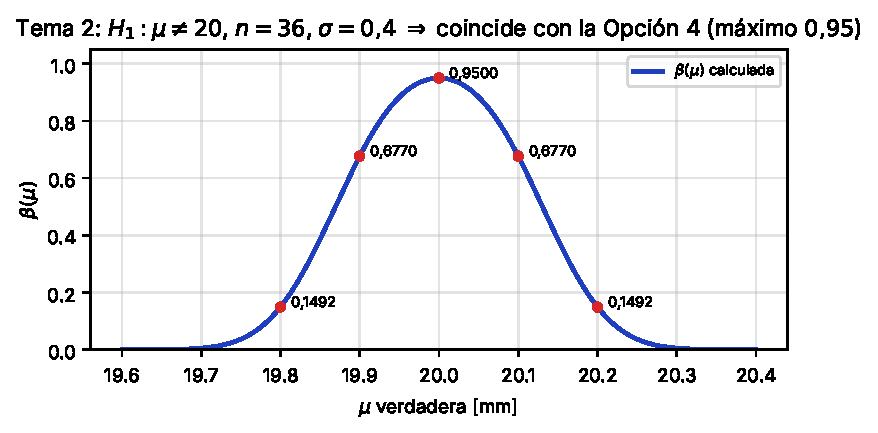
\includegraphics[width=0.78\textwidth]{fig/t2beta.pdf}
\end{figure}
\begin{resp}
\textbf{Opción 4.} Es una campana \textbf{simétrica} alrededor de $\mu_0=20$ (prueba bilateral), con máximo $1-\alpha=0{,}95$ en $\mu=20$, y vale $\approx0{,}15$ en 19,8 y en 20,2.
Se descartan: 2 (campana con máximo 0,90, que correspondería a $\alpha=0{,}10$); 1, 3, 5 y 6 (monótonas: corresponden a pruebas unilaterales).
\end{resp}

\inciso{d) IC del 95\,\% para $\mu$}
Con $\sigma$ conocido y $n=36$:
\[
20{,}15\pm1{,}96\,(0{,}0667)=20{,}15\pm0{,}1307\ \Rightarrow\ \res{20{,}0193\le\mu\le20{,}2807\ \text{mm}}
\]
El valor 20 \textbf{no} está en el intervalo, lo que coincide con el rechazo de b). Por la dualidad, una prueba bilateral con nivel $\alpha$ rechaza $H_0$ exactamente cuando $\mu_0$ queda fuera del IC del $(1-\alpha)$.

\inciso{e) Tamaño de muestra}
Se pide potencia 0,80 (o sea $\beta=0{,}20$) cuando $\mu=20{,}1$ ($\delta=0{,}1$), con la misma prueba bilateral y $\alpha=0{,}05$. Los valores críticos son $z_{0,025}=1{,}96$ y $z_{0,20}=0{,}8416$:
\[
n\approx\frac{(z_{\alpha/2}+z_\beta)^2\sigma^2}{\delta^2}=\frac{(1{,}96+0{,}8416)^2\,(0{,}40)^2}{0{,}1^2}=125{,}59\ \Rightarrow\ \res{n=126}
\]
Comprobación: con $n=126$ la potencia es 0,8013 \checkmark; con $n=125$ sería 0,7982, que no alcanza.
